\begin{frame}{Génération de surface de contacts}
    \begin{itemize}
        \item Les algorithmes présentés ne calculent qu’un point de contact.
        \item C’est rarement suffisant et provoque des vibrations:
    \end{itemize}
    \begin{center}
        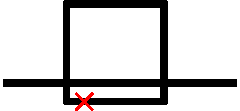
\includegraphics[scale=0.5]{acc_contact_1}
        \pause
        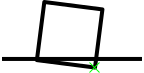
\includegraphics[scale=0.5]{contact_2}
        \pause
        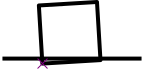
\includegraphics[scale=0.5]{contact_3}
        \pause
        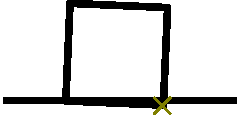
\includegraphics[scale=0.5]{contact_4}
        \pause
        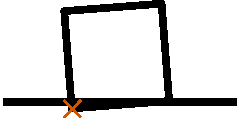
\includegraphics[scale=0.5]{contact_5}
        \pause
    \end{center}

    Solution: accumuler les contacts sur plusieurs frames en maximisant la
    dispersion des points.
    \pause
    \begin{center}
        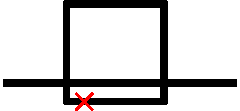
\includegraphics[scale=0.5]{acc_contact_1}
        \pause
        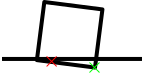
\includegraphics[scale=0.5]{acc_contact_2}
        \pause
        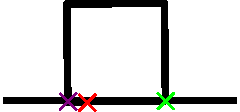
\includegraphics[scale=0.5]{acc_contact_3}
        \pause
        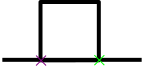
\includegraphics[scale=0.5]{acc_contact_4}
    \end{center}
\end{frame}

\begin{frame}{La Broad Phase}
    \begin{itemize}
        \item Tester les $n * (n + 1) / 2$ paires de collisions est impraticable.
        \item Il faut tester les collisions de manières approximatives avant de
            faire les calculs les plus lourds!
    \end{itemize}
    \pause
    \begin{description}
        \item[Volumes anglobants:]
    \end{description}
    \begin{center}
        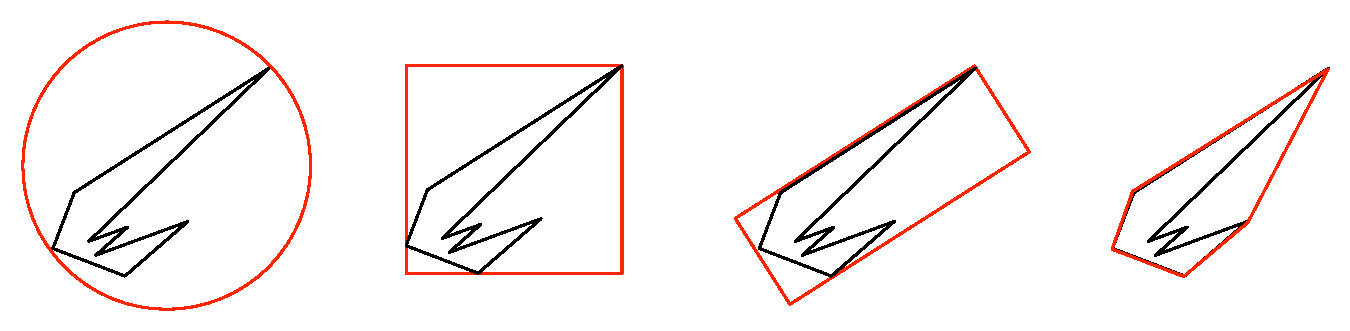
\includegraphics[scale=0.5]{bounding_volumes}
    \end{center}
\end{frame}

\begin{frame}{La Broad Phase}
    Les volumes anglobants peuvent former un arbre.
    \begin{center}
            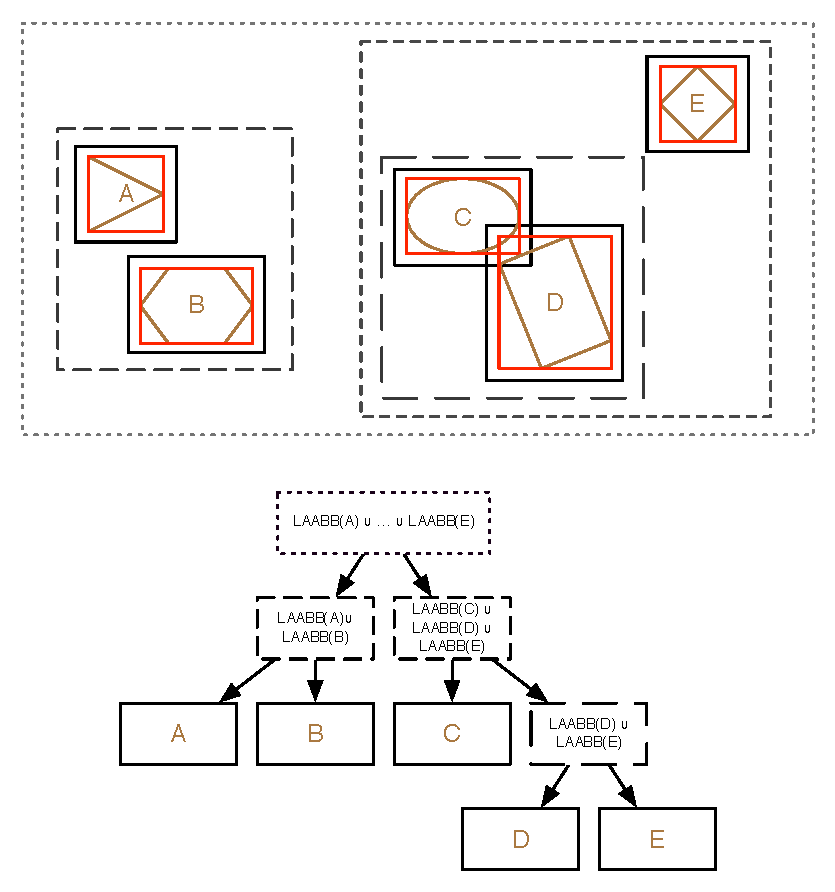
\includegraphics[scale=0.5]{AABB_tree}
    \end{center}
\end{frame}

\begin{frame}{L'endormissement}
    \begin{itemize}
        \item La plupart du temps l’utilisateur n’intéragit qu’avec
            peu d’objets. Pourquoi simuler la physique des objets immobiles?
        \pause
        \item Il faut détecter les groupes d’objets immobiles et les
            ignorer.
    \end{itemize}
        \pause
    \begin{description}
        \item[Pseudo énergie cinétique:]\mbox{}
            \[
                E(t) = m * v^2 + \boldsymbol\omega^t * I * \boldsymbol\omega
            \]
        \pause
    \item[Recency Weighted Average:]\mbox{}
        \[
            \begin{array}{lcl}
                E_{rwa}(0) & = & E_{\text{max}}\\
                E_{rwa}(t + \Delta t) & = & \alpha * E_{rwa}(t) + (1 - \alpha) * E(t + \Delta t)\\
                E_{rwa}(t + \Delta t) & = & \min(E_{rwa}(t + \Delta t), E_{\text{max}})\\
            \end{array}
        \]
    \end{description}
    \pause
    Si $E_{rwa}$ est trop bas pour un groupe d’objets en contact, ils peuvent
    être désactivés (aka. endormis).
\end{frame}
